%%%%%%%%%%%%%%%%%%%%%%%%%%%%%%%%%%%%%%%%%
% Beamer Presentation
% LaTeX Template
% Version 1.0 (10/11/12)
%
% This template has been downloaded from:
% http://www.LaTeXTemplates.com
%
% License:
% CC BY-NC-SA 3.0 (http://creativecommons.org/licenses/by-nc-sa/3.0/)
%
%%%%%%%%%%%%%%%%%%%%%%%%%%%%%%%%%%%%%%%%%

%----------------------------------------------------------------------------------------
%	PACKAGES AND THEMES
%----------------------------------------------------------------------------------------

\documentclass{beamer}

\mode<presentation> {

% The Beamer class comes with a number of default slide themes
% which change the colors and layouts of slides. Below this is a list
% of all the themes, uncomment each in turn to see what they look like.

%\usetheme{default}
%\usetheme{AnnArbor}
%\usetheme{Antibes}
%\usetheme{Bergen}
%\usetheme{Berkeley}
%\usetheme{Berlin}
%\usetheme{Boadilla}
%\usetheme{CambridgeUS}
%\usetheme{Copenhagen}
%\usetheme{Darmstadt}
%\usetheme{Dresden}
%\usetheme{Frankfurt}
%\usetheme{Goettingen}
%\usetheme{Hannover}
%\usetheme{Ilmenau}
%\usetheme{JuanLesPins}
%\usetheme{Luebeck}
%\usetheme{ClassyCharcoal}
%\usetheme{Malmoe}
%\usetheme{Marburg}
%\usetheme{Montpellier}
%\usetheme{PaloAlto}
%\usetheme{Pittsburgh}
\usetheme{Rochester}
%\usetheme{Singapore}
%\usetheme{Szeged}
%\usetheme{Warsaw}

% As well as themes, the Beamer class has a number of color themes
% for any slide theme. Uncomment each of these in turn to see how it
% changes the colors of your current slide theme.

%\usecolortheme{albatross}
%\usecolortheme{beaver}
%\usecolortheme{beetle}
%\usecolortheme{crane}
%\usecolortheme{dolphin}
%\usecolortheme{dove}
%\usecolortheme{fly}
%\usecolortheme{lily}
%\usecolortheme{orchid}
%\usecolortheme{rose}
%\usecolortheme{seagull}
%\usecolortheme{seahorse}
\usecolortheme{whale}
%\usecolortheme{wolverine}

%\setbeamertemplate{footline} % To remove the footer line in all slides uncomment this line
\setbeamertemplate{footline}[frame number] % To replace the footer line in all slides with a simple slide count uncomment this line

%\setbeamertemplate{navigation symbols}{} % To remove the navigation symbols from the bottom of all slides uncomment this line
}

\usepackage{mathtools}
\usepackage{subfig}
\usepackage{graphicx} % Allows including images
\graphicspath{{figures/pdf/}{figures/eps/}{figures/jpg/}}
\usepackage{booktabs} % Allows the use of \toprule, \midrule and \bottomrule in tables
\usepackage{algorithmic}
\usepackage{epstopdf}
\usepackage{tikz}
\usepackage[T1]{fontenc}

\usepackage{float}
\newfloat{algorithm}{t}{lop}
\floatname{algorithm}{Algorithm}

\usepackage{accents}
\newcommand{\ubar}[1]{\underaccent{\bar}{#1}}

\usepackage{amssymb}
\usepackage{cleveref}

\setbeamercovered{transparent}
%\useoutertheme{infolines}
\beamertemplatenavigationsymbolsempty

\pgfdeclareimage[height=0.5cm]{logo}{ut2}
\logo{\pgfuseimage{logo}}

\usepackage{array}
\newcolumntype{L}[1]{>{\raggedright\let\newline\\\arraybackslash\hspace{0pt}}m{#1}}

\usepackage[labelsep=colon]
                %labelfont={sf,bf},
                %textfont=sf]
               {caption}

\newenvironment{figure*}%
{\begin{figure}}
{\end{figure}}

\pdfmapfile{+sansmathaccent.map}

%----------------------------------------------------------------------------------------
%	TITLE PAGE
%----------------------------------------------------------------------------------------

\title[Computational Algorithms for Flight Safety]{Development of Adaptive Computational Algorithms for Manned and Unmanned Flight Safety}

\author{Colin P.~Elkin, PhD Candidate} % Your name
\institute[UT] % Your institution as it will appear on the bottom of every slide, may be shorthand to save space
{
Committee Chair: Dr.~Vijay Devabhaktuni \\
Committee Member: Dr.~Mansoor Alam \\ 
Committee Member: Dr.~Ahmad Javaid \\ 
Committee Member: Dr.~Devinder Kaur \\
Committee Member: Dr.~Weiqing Sun \\ 
Committee Member: Dr.~Lawrence Thomas \\
\medskip
Department of EECS, The University of Toledo 
}
\date{November 5th, 2018} % Date, can be changed to a custom date

\begin{document}

\begin{frame}
\titlepage % Print the title page as the first slide
\end{frame}

\begin{frame}
\frametitle{Overview} % Table of contents slide, comment this block out to remove it
\tableofcontents % Throughout your presentation, if you choose to use \section{} and \subsection{} commands, these will automatically be printed on this slide as an overview of your presentation
\end{frame}

%----------------------------------------------------------------------------------------
%	PRESENTATION SLIDES
%----------------------------------------------------------------------------------------

%------------------------------------------------
\section{Introduction} 
%------------------------------------------------

%------------------------------------------------

\begin{frame}
\frametitle{Overview: Airline Safety Issues}
\begin{columns}[c]
\column{.45\textwidth} 
\includegraphics[width=\textwidth]{flight}
%\includegraphics<2>[width=\textwidth]{frame3-2.eps}
%\includegraphics<3>[width=\textwidth]{frame3-3.eps}
%\includegraphics<4>[width=\textwidth]{frame3-4.eps}
\column{.45\textwidth} 
\begin{itemize}
\item{Important human factor: high mental workload}
\item{Pilots work under high levels of multitasking}
\item{Risk of mental overload}
\end{itemize}
\end{columns}
\end{frame}

\begin{frame}
\frametitle{Overview: Airline Safety Issues}
\begin{columns}[c]
\column{.45\textwidth} 
\includegraphics[width=\textwidth]{flight}
%\includegraphics<2>[width=\textwidth]{frame3-2.eps}
%\includegraphics<3>[width=\textwidth]{frame3-3.eps}
%\includegraphics<4>[width=\textwidth]{frame3-4.eps}
\column{.45\textwidth} 
\begin{itemize}
\item{Some automation have been implemented to ease the burden of overload}
\item{Can result in mental underload}
\item{Impacts ability to react to sudden events}
\item{Example: driver overload vs. underload}
\end{itemize}
\end{columns}
\end{frame}

\begin{frame}
\frametitle{Overview: Airline Safety Issues}
\begin{columns}[c]
\column{.45\textwidth} 
\includegraphics[width=\textwidth]{flight}
%\includegraphics<2>[width=\textwidth]{frame3-2.eps}
%\includegraphics<3>[width=\textwidth]{frame3-3.eps}
%\includegraphics<4>[width=\textwidth]{frame3-4.eps}
\column{.45\textwidth} 
\begin{itemize}
\item{Flight safety has improved, but goal is always to achieve near 100\% safety}
\item{Goal: examine human aspects of safety by optimal cognitive workload}
\end{itemize}
\end{columns}
\end{frame}

\begin{frame}
\frametitle{UAVs in Shared Airspace: a New Frontier}
\begin{itemize}
\item{Before 2012: mostly used by hobbyists and military}
\item{Today: broader and more commercial applications}
\item{Need for UAVs to integrate into shared airspace}
\item{Thus, UAV safety will be a growing concern}
\end{itemize}
\includegraphics[width=\textwidth]{overview}
\end{frame}

\begin{frame}
\frametitle{Research Objectives and Process}
\includegraphics[width=\textwidth]{process}
\end{frame}

%\begin{frame}
%\frametitle{Problem Statement}
%\begin{columns}[c]
%\column{.32\textwidth} 
%\includegraphics[width=.8\textwidth]{phone}
%\column{.55\textwidth} 
%\includegraphics[width=\textwidth]{fire}
%\end{columns}
%\pause\begin{block}{Goals and Objectives of this Research}
%{To develop new methods for finding a Node's location in a Wireless Sensor Network with both High Accuracy and Low Computational Cost}
%\end{block}
%\end{frame}

%\begin{frame}
%\frametitle{Established Localization Techniques}
%\includegraphics<1>[width=.8\textwidth]{algs}
%\includegraphics<2>[width=.8\textwidth]{algs1}
%\end{frame}
%
%\begin{frame}
%\frametitle{Received Signal Strength (RSS)}
%\begin{center}
%\includegraphics[width=.7\linewidth]{rss.pdf}
%\end{center}
%\begin{itemize}
%\item{Defined as measured power or square of signal strength}
%\item{Most vital property: RSS is inversely proportional to distance}
%\item{Estimation done by trilateration}
%\end{itemize}
%\end{frame}
%
%\begin{frame}
%\frametitle{Angle of Arrival (AOA)}
%\begin{center}
%\includegraphics[width=.7\linewidth]{aoa.pdf}
%\end{center}
%\begin{itemize}
%\item{Measures angles at 2+ receivers}
%\item{Estimation done through triangulation}
%\item{Based on TDOA measurements}
%\end{itemize}
%\end{frame}
%
%\begin{frame}
%\frametitle{Other Localization Techniques}
%\begin{table}
%\renewcommand{\arraystretch}{1.3}
%\begin{tabular}{L{2cm} L{2cm} L{2cm} L{2cm}}
%\toprule
%\textbf{Technique} & \textbf{Overview} & \textbf{Advantages} & \textbf{Disadvantages} \\ 
%\midrule
%Genetic Algorithm (GA) & Evolutionary population of candidate solutions & Ideal for large-scale search problems & Premature convergence \\ 
%Particle Swarm Optimization (PSO) & Based on particles and movements & Ideal for problems with real values & Expensive computational runtime \\ 
%\bottomrule
%\end{tabular}
%\caption{Summary of global, biologically inspired localization techniques.}
%\end{table}
%\end{frame}
%
%\begin{frame}
%\frametitle{Overview of DS Theory}
%\begin{center}
%\includegraphics[width=.2\linewidth]{prob}
%\end{center}
%\begin{itemize}
%\item{Divergence from Bayesian Probability}
%\item{Based on concept of ignorance}
%\item{Bayesian probability combines internal factors}
%\item{DS Theory uses external factors}
%\end{itemize}
%\end{frame}
%
%\begin{frame}
%\frametitle{Example: Broken Chair}
%\begin{table}
%\begin{tabular}{l l }
%\toprule
%\textbf{Component} & \textbf{Failure Probability}\\
%\midrule
%Wheels & 60\% chance of breaking \\
%Back & 20\% chance of falling apart \\
%Arm Rests & 40\% chance of falling off \\
%\bottomrule
%\end{tabular}
%\caption{Failure analysis of each chair component}
%\end{table}
%
%\pause
%\begin{block}{Probability of Total Failure}
%{$.6 \times .4 \times .2 = .048$ or 4.8\%}
%\end{block}
%\end{frame}
%
%\begin{frame}
%\frametitle{Example: Broken Chair}
%\begin{table}
%\begin{tabular}{l l l l}
%\toprule
%\textbf{Expert} & \textbf{Lower Bound} & \textbf{Upper Bound} & \textbf{Confidence}\\
%\midrule
%A & 11 & 18 & .4 \\
%B & 14 & 21 & .4 \\
%C & 10 & 20 & .2 \\
%\bottomrule
%\end{tabular}
%\caption{Failure analysis by three experts}
%\end{table}
%
%\begin{itemize}
%\pause\item{Expected Value Range of 100\% Failure: 12-19.6 Days}
%\item{Most Plausible Time of 100\% Failure: 14 Days}
%\item{Most Believable Time of 100\% Failure: 21 Days}
%\end{itemize}
%\end{frame}
%
%\begin{frame}
%\frametitle{Applications of and Motivations for DS Theory}
%\begin{figure*}\centering
%\subfloat[Failure Analysis \label{car}]
%        {\includegraphics[width=0.22\textwidth]{broken_car}}
%   % \hfill
%\subfloat[Robot Sensor Fusion\label{robot}]
%         {\includegraphics[width=0.22\textwidth]{robot}}
%\subfloat[GPS/INS Data Fusion \label{gps}]
%         {\includegraphics[width=0.22\textwidth]{gps}}
%   % \hfill
%\subfloat[Wireless Sensor Networks \label{wsn}]
%        {\includegraphics[width=0.22\textwidth]{wsn}}
%    \label{apps}
%    \end{figure*}
%\begin{itemize}
%\item{No need to train data}
%\item{Fast and computationally efficient}
%\end{itemize}
%\end{frame}

\section{Cognitive Workload Assessment}

%\subsection{Introduction and Background}

%\begin{frame}
%\frametitle{First Proposed Algorithm}
%\begin{itemize}
%\item{Does the set of measurements belong to the county?}
%\end{itemize}
%\begin{center}
%\includegraphics[width=.8\textwidth]{classifier2}
%\end{center}
%\end{frame}


\begin{frame}
\frametitle{Cognitive Workload Assessment}
\begin{block}{Problem Statement}
{The aim of this phase of the research is to perform an analysis of alternatives of the machine learning approaches that are currently used for assessing cognitive workload.}
\end{block}
\begin{center}
\includegraphics[width=.9\textwidth]{cw}
\end{center}
\end{frame}

\begin{frame}
\frametitle{Experimental Process}
\begin{center}
\includegraphics[width=.65\textwidth]{exp-fig}
\end{center}
\end{frame}

\begin{frame}
\frametitle{Approach: Data Acquisition}
\includegraphics[width=\textwidth]{data}
\end{frame}

\begin{frame}
\frametitle{Approach: Data Acquisition II}
\begin{center}
\includegraphics[width=.75\textwidth]{saphyre}
\end{center}
\end{frame}

\begin{frame}
\frametitle{Approach: Data Acquisition - Arithmetic}
\includegraphics[width=\textwidth]{nata-io}
\end{frame}

\begin{frame}
\frametitle{Approach: Data Acquisition - Visual Matching}
\includegraphics[width=\textwidth]{vismatch-io}
\end{frame}

\begin{frame}
\frametitle{Approach: Data Acquisition - DEAP}
\includegraphics[width=\textwidth]{deap-io}
\end{frame}

\begin{frame}
\frametitle{Experimental Setup}
\begin{center}
\includegraphics[width=.2\textwidth]{python}
\end{center}
\begin{itemize}
\item{Programmed in Python using scikit-learn toolkit for built-in ML tools}
\item{Tested under multiple method-specific parameters}
\item{Used iterative combinations of other parameters to show how results vary in three dimensions}
\item{Results presented as averages of 10 independent experiments}
\end{itemize}
\end{frame}

\begin{frame}
\frametitle{SAPHYRE Results}
\begin{columns}[c]
\column{.5\textwidth} 
\begin{center}
ANN Accuracy
\end{center}
\includegraphics[width=\textwidth]{saphyre/ANN/sgd_val}
\column{.5\textwidth} 
\begin{center}
RF Accuracy
\end{center}
\includegraphics[width=\textwidth]{saphyre/RFR/entropy_val}
\end{columns}
%\pause\begin{block}{Goals and Objectives of this Research}
%{To develop new methods for finding a Node's location in a Wireless Sensor Network with both High Accuracy and Low Computational Cost}
%\end{block}
\end{frame}

\begin{frame}
\frametitle{SAPHYRE Results II}
\begin{columns}[c]
\column{.5\textwidth} 
\begin{center}
ANN Runtime
\end{center}
\includegraphics[width=\textwidth]{saphyre/ANN/sgd_runtime}
\column{.5\textwidth} 
\begin{center}
RF Runtime
\end{center}
\includegraphics[width=\textwidth]{saphyre/RFR/entropy_runtime}
\end{columns}
%\pause\begin{block}{Goals and Objectives of this Research}
%{To develop new methods for finding a Node's location in a Wireless Sensor Network with both High Accuracy and Low Computational Cost}
%\end{block}
\end{frame}

\begin{frame}
\frametitle{Overview of ML Analysis}
\begin{table}[!t]
%\caption{Summary of technique comparison on all data.}
\renewcommand{\arraystretch}{1.3}
\centering
\resizebox{\textwidth}{!}
{\begin{tabular}{*{5}{l}}
\toprule
Technique & Arithmetic & DEAP & Visual Matching & SAPHYRE \\ \midrule
ANN SGD & Wide range of results & Best in most metrics & Best runtime & Widest range of results \\
ANN LBFGS & Wide range of results & Best in most metrics & Nothing noteworthy & Highest max.~runtime \\
KNN Uniform & Most susceptible to overfitting & Worst max.~runtime & Overfitting & Nothing noteworthy \\
KNN Distance & Most susceptible to overfitting & Second worst max.~runtime & Overfitting & Nothing noteworthy \\
SVM Linear & Worst in all metrics & Worst in most metrics & Nothing noteworthy & Nothing noteworthy \\
SVM RBF & Worst maximum runtime & Worst runtime & Worst runtime & Nothing noteworthy \\
DT Gini & Best in all metrics & Nothing noteworthy & Best in most metrics & Nothing noteworthy \\
DT Entropy & Best in all except runtime & Nothing noteworthy & Second best in most metrics & Best runtime \\
RF Gini & Second best in most metrics & Nothing noteworthy & Overfitting & Best max.~accuracy \\
RF Entropy & Third best in most metrics & Nothing noteworthy & Overfitting & Best in most metrics \\ \bottomrule
\end{tabular}}
\end{table}
\end{frame}

\begin{frame}
\frametitle{Overview of ML Analysis}
\begin{table}[!t]
%\caption{Summary of technique comparison on all data.}
\renewcommand{\arraystretch}{1.3}
\centering
\resizebox{\textwidth}{!}
{\begin{tabular}{*{5}{l}}
\toprule
Technique & Arithmetic & DEAP & Visual Matching & SAPHYRE \\ \midrule
ANN SGD & Wide range of results & \textbf{Best in most metrics} & Best runtime & Widest range of results \\
ANN LBFGS & Wide range of results & \textbf{Best in most metrics} & \textit{Nothing noteworthy} & Highest max.~runtime \\
KNN Uniform & Most susceptible to overfitting & Worst max.~runtime & Overfitting & \textit{Nothing noteworthy} \\
KNN Distance & Most susceptible to overfitting & Second worst max.~runtime & Overfitting & \textit{Nothing noteworthy} \\
SVM Linear & Worst in all metrics & Worst in most metrics & \textit{Nothing noteworthy} & \textit{Nothing noteworthy} \\
SVM RBF & Worst maximum runtime & Worst runtime & Worst runtime & \textit{Nothing noteworthy} \\
DT Gini & \textbf{Best in all metrics} & \textit{Nothing noteworthy} & \textbf{Best in most metrics} & \textit{Nothing noteworthy} \\
DT Entropy & \textbf{Best in all except runtime} & \textit{Nothing noteworthy} & \textbf{Second best in most metrics} & Best runtime \\
RF Gini & Second best in most metrics & \textit{Nothing noteworthy} & Overfitting & \textbf{Best max.~accuracy} \\
RF Entropy & Third best in most metrics & \textit{Nothing noteworthy} & Overfitting & \textbf{Best in most metrics} \\ \bottomrule
\end{tabular}}
\end{table}
\end{frame}

\begin{frame}
\frametitle{Next Steps}
\includegraphics[width=\textwidth]{next-steps}
\end{frame}

\section{Adaptive Workload Prediction}

\begin{frame}
\frametitle{Adaptive Workload Prediction - Background}
\begin{table}[!t]
%\caption{Summary of cognitive workload datasets and results.}
\renewcommand{\arraystretch}{1.3}
\centering
\resizebox{\textwidth}{!}
{\begin{tabular}{*{5}{l}}
\toprule
Dataset & No.~Inputs & No.~Classifications & Best Method & Optimal Parameters \\ \midrule
Arithmetic & 3 & 5 & DT & gini, 9 for split, 2 for leaf\\
Visual Matching & 66 & 3 & DT & gini, 9 for split, 2 for leaf \\
DEAP & 42 & 40 & ANN & SGD, 7 neurons, 2 layers \\
SAPHYRE & 16 & 165 & RF & entropy, 7 for split, 10 for leaf \\ \bottomrule
\end{tabular}}
\end{table}
\end{frame}

\begin{frame}
\frametitle{Adaptive Workload Prediction - Background}
\begin{table}[!t]
%\caption{Summary of cognitive workload datasets and results.}
\renewcommand{\arraystretch}{1.3}
\centering
\resizebox{\textwidth}{!}
{\begin{tabular}{*{5}{l}}
\toprule
Dataset & No.~Inputs & No.~Classifications & Best Method & Optimal Parameters \\ \midrule
Arithmetic & Lo & Lo & DT & gini, 9 for split, 2 for leaf\\
Visual Matching & Hi & Lo & DT & gini, 9 for split, 2 for leaf \\
DEAP & Hi & Hi & ANN & SGD, 7 neurons, 2 layers \\
SAPHYRE & Lo & Hi & RF & entropy, 7 for split, 10 for leaf \\ \bottomrule
\end{tabular}}
\end{table}
\end{frame}

\begin{frame}
\frametitle{Adaptive Algorithm - Single Selection}
\begin{center}
\scalebox{0.8}{
\begin{minipage}{\linewidth}
\begin{algorithm}[H]
\begin{algorithmic}[1]
\STATE train\_in, val\_in, train\_out, val\_out $\leftarrow$ all possible input and output data	
\IF{number of output classifications < 20}
	\STATE create DT classifier
\ELSE
	\IF{number of inputs > 20}
		\STATE create ANN classifier
	\ELSE
		\STATE create RF classifier
	\ENDIF
\ENDIF		
\STATE train selected classifier
\FORALL{validation time steps}
	\STATE get validation accuracy for all time steps evaluated thus far
\ENDFOR
\RETURN val\_accuracy, method, runtime, train\_accuracy
\label{full-alg-dagsi2-1}
\end{algorithmic}
\caption{Pseudocode of single selection process.} 
\label{full-alg-dagsi2-1}
\end{algorithm}	
\end{minipage} }
\end{center}
\end{frame}

\begin{frame}
\frametitle{Adaptive Algorithm - Dynamic Selection}
\begin{center}
\scalebox{0.65}{
\begin{minipage}{\linewidth}
\begin{algorithm}[H]
\begin{algorithmic}[1]
\STATE train\_in, val\_in, train\_out, val\_out $\leftarrow$ all possible input and output data	
\STATE create and train ANN, DT, and RF classifiers
\IF{number of output classifications < 20}
	\STATE select DT
\ELSE
	\IF{number of inputs > 20}
		\STATE select ANN
	\ELSE
		\STATE select RF
	\ENDIF
\ENDIF		
\FORALL{validation time steps}
	\STATE get validation accuracy from selected method for all completed time steps
	\IF{accuracy is lower than that of another method}
		\STATE select method with highest accuracy
	\ENDIF	
\ENDFOR		
\RETURN val\_accuracy, method, runtime, train\_accuracy
\label{full-alg-dagsi2-2}
\end{algorithmic}
\caption{Pseudocode of dynamic selection process.} 
\label{full-alg-dagsi2-2}
\end{algorithm}
\end{minipage}	}
\end{center}
\end{frame}

\begin{frame}
\frametitle{Experimental Setup}
\begin{center}
\includegraphics[width=.2\textwidth]{python}
\end{center}
\begin{itemize}
\item{Programmed in Python using scikit-learn toolkit for built-in ML tools}
\item{Tested per dataset, per algorithm, and per validation ratio (25\%, 66\%)}
\item{Results presented as averages of 10 independent experiments}
\end{itemize}
\end{frame}

\begin{frame}
\frametitle{Single Selection Results}
\begin{table}[!t]
%\caption{Summary of training accuracy, validation accuracy, and computational runtime under the single selection algorithm with 25\% of samples used for validation.}
\renewcommand{\arraystretch}{1.3}
\centering
%\resizebox{\textwidth}{!}
{\begin{tabular}{*{5}{l}}
\toprule
Metric & Arithmetic & Visual Matching & SAPHYRE \\ \midrule
Training Accuracy & .999 & .967 & .995 \\
Validation Accuracy & .999 & .902 & .989 \\
Runtime (s) & 12.1 & 36.5 & 129 \\ \bottomrule
\end{tabular}}
\end{table}
\end{frame}

\begin{frame}
\frametitle{Dynamic Selection Results}
\begin{table}[!t]
%\caption{Summary of training accuracy, validation accuracy, and computational runtime under the dynamic selection algorithm with 25\% of samples used for validation.}
\renewcommand{\arraystretch}{1.2}
\centering
%\resizebox{\textwidth}{!}
{\begin{tabular}{*{10}{l}}
\toprule
Metric & Arithmetic & Visual Matching & SAPHYRE \\ \midrule
RF Train.~Accuracy & .998 & .845 & .995 \\
DT Train.~Accuracy & .999 & .974 & .997 \\
ANN Train.~Accuracy & .444 & .724 & .161 \\
Validation Accuracy & .999 & .902 & .991 \\
Runtime (s) & 134 & 147 & 241 \\ \bottomrule
\end{tabular}}
\label{dyn-all}
\end{table}
\end{frame}

\begin{frame}
\frametitle{Dynamic Selection Results per Sample - 25\% Validation}
\begin{columns}[c]
\column{.33\textwidth} 
\begin{center}
Arithmetic data
\end{center}
\includegraphics[width=\textwidth]{switching/nata/0.25/nata25}

\column{.33\textwidth} 
\begin{center}
Visual matching data
\end{center}
\includegraphics[width=\textwidth]{switching/vismatch/0.25/vismatch25}

\column{.33\textwidth}
\begin{center}
SAPHYRE data
\end{center}
\includegraphics[width=\textwidth]{switching/saphyre/0.25/saphyre25}
\end{columns}

\end{frame}

\begin{frame}
\frametitle{Dynamic Selection Results per Sample - 66\% Validation}
\begin{columns}[c]
\column{.33\textwidth} 
\begin{center}
Arithmetic data
\end{center}
\includegraphics[width=\textwidth]{switching/nata/0.66/nata66}

\column{.33\textwidth} 
\begin{center}
Visual matching data
\end{center}
\includegraphics[width=\textwidth]{switching/vismatch/0.66/vismatch66}

\column{.33\textwidth}
\begin{center}
SAPHYRE data
\end{center}
\includegraphics[width=\textwidth]{switching/saphyre/0.66/saphyre66}
\end{columns}

\end{frame}

\section{Performance Assessment of Unmanned Aerial Vehicles}

\begin{frame}
\frametitle{Autonomous UAV Behavior}
\begin{columns}
\column{.66\textwidth}
% bullet points and block
\begin{itemize}
\item Autonomous UAV behavior can be surprising to operators
\item Need to improve transparency and understandability of autonomous behavior
\item Also a need to reduce surprises from the start with improved predictions to weigh against outcomes
\end{itemize}
\begin{block}{Problem Statement}
{The aim of this phase of the research is to use machine learning and data fusion to enhance the prediction of UAV behavior and explain the unpredictable.}
\end{block}

\column{.33\textwidth}
\includegraphics[width=\textwidth]{epex}
\end{columns}
\end{frame}

\begin{frame}
\frametitle{Inclusion of Data Fusion}
\includegraphics[width=\textwidth]{data-fusion}
\end{frame}

\begin{frame}
\frametitle{Proposed ANN+DSET Algorithm}
\includegraphics[width=\textwidth]{dset}
\end{frame}

\begin{frame}
\frametitle{Experimental Setup}
\begin{center}
\includegraphics[width=.2\textwidth]{ml}
\end{center}
\begin{itemize}
\item Programmed in MATLAB
\item Evaluated on a dataset of six UAVs over 695 seconds leading up to a crash
\item Compared against a standard ANN to test the advantages/disadvantages of including DSET-based sensor fusion
\item Also compared against Extended Kalman Filter and Unscented Kalman Filter
\item Results given as the average of 10 independent trials for consistency
\end{itemize}
\end{frame}

\begin{frame}
\frametitle{Methods to Compare}
\begin{columns}
\column{.5\textwidth}
\includegraphics[width=\textwidth]{io}
\begin{itemize}
\item Multi-layer Perceptron (MLP)
\item Used for regression rather than classification
\item Trained with Ant Colony Optimization
\item No explicit data fusion
\end{itemize}

\column{.5\textwidth}
\includegraphics[width=\textwidth]{kf-fig}
\begin{itemize}
\item Extended Kalman filter (EKF) and unscented Kalman filter (UKF)
\item Uses equations derived from UAV dynamic models
\item Differ from one another in amount of linearization involved
\end{itemize}
\end{columns}
\end{frame}


\begin{frame}
\frametitle{Comparison Results}
\begin{columns}[c]
\column{.5\textwidth} 
\begin{center}
One UAV at a time (average)
\end{center}
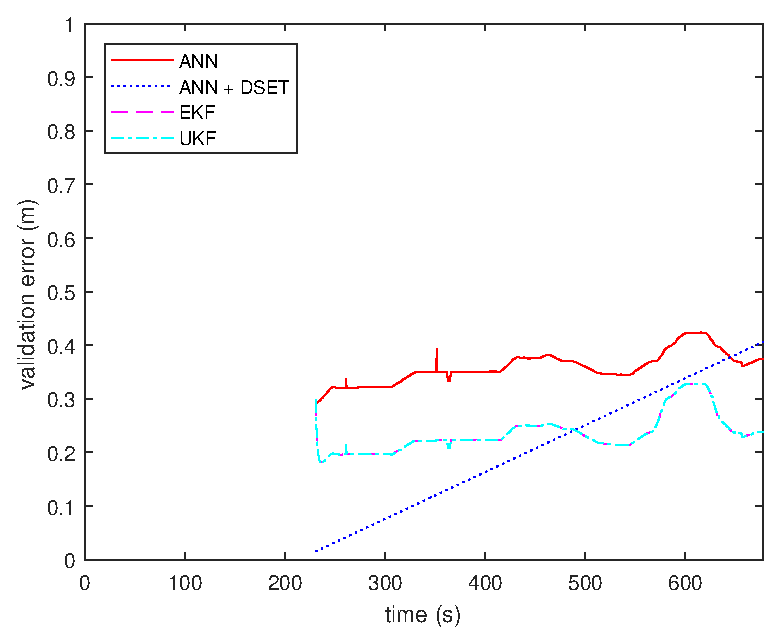
\includegraphics[width=\textwidth]{100-onefull.eps}
\column{.5\textwidth} 
\begin{center}
All UAVs evaluated together
\end{center}
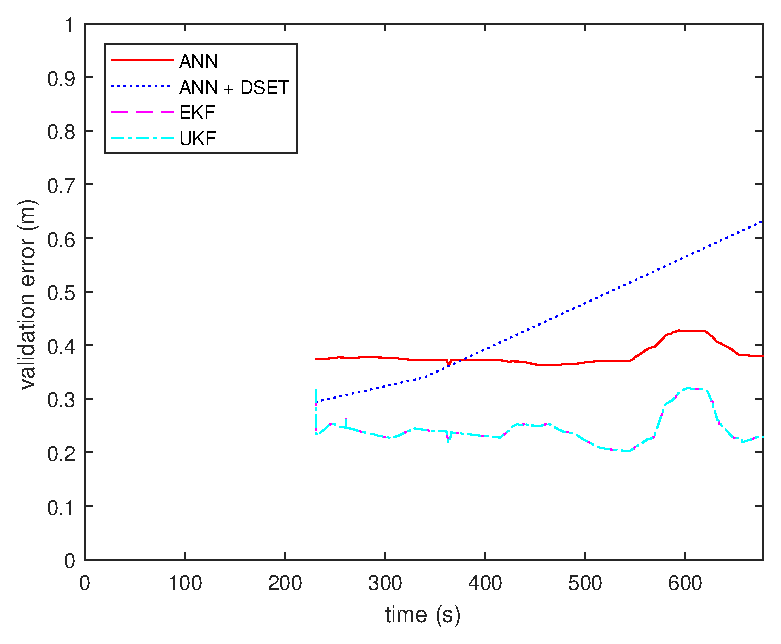
\includegraphics[width=\textwidth]{100-multifull.eps}
\end{columns}
%\pause\begin{block}{Goals and Objectives of this Research}
%{To develop new methods for finding a Node's location in a Wireless Sensor Network with both High Accuracy and Low Computational Cost}
%\end{block}
\end{frame}

\begin{frame}
\frametitle{Next Steps}
\includegraphics[width=\textwidth]{next-steps1}
\end{frame}

\section{Adaptive Trajectory Prediction}

\begin{frame}
\frametitle{Adaptive Trajectory Prediction}
\begin{center}
\includegraphics[width=.6\textwidth]{switching1}
\end{center}
\end{frame}

\begin{frame}
\frametitle{Experimental Setup}
\begin{center}
\includegraphics[width=.2\textwidth]{ml}
\end{center}
\begin{itemize}
\item Programmed in MATLAB
\item Evaluated on a dataset of six UAVs over 695 seconds leading up to a crash
\item Results given as the average of 10 independent trials for consistency
\end{itemize}
\end{frame}

\begin{frame}
\frametitle{Comparison Results}
\begin{columns}[c]
\column{.5\textwidth} 
\begin{center}
One UAV at a time (average)
\end{center}
\includegraphics[width=\textwidth]{100-onefulls.eps}
\column{.5\textwidth} 
\begin{center}
All UAVs evaluated together
\end{center}
\includegraphics[width=\textwidth]{100-multifulls.eps}
\end{columns}
%\pause\begin{block}{Goals and Objectives of this Research}
%{To develop new methods for finding a Node's location in a Wireless Sensor Network with both High Accuracy and Low Computational Cost}
%\end{block}
\end{frame}

\section{Conclusions and Future Work}

\begin{frame}
\frametitle{Publications}
[1] C.~Elkin, B.~Marinier, A.~Javaid, D.~Kaur, V.~Devabhaktuni, and J.~Zaientz, ``Computational approaches for optimal manned and unmanned flight safety: a survey,'' Information Sciences (Under preparation)

[2] C.~Elkin, B.~Marinier, A.~Javaid, D.~Kaur, V.~Devabhaktuni, and J.~Zaientz, ``Prediction of unmanned aerial vehicle behavior through a combination of Dempster-Shafer and artificial neural network sensor
fusion,'' Expert Systems with Applications (Under revision) 
\end{frame}

\begin{frame}
\frametitle{Publications II}
[3] C.~Elkin and V.~Devabhaktuni, ``Analysis of Alternatives for Neural Network Training Techniques in Assessing Cognitive Workload,'' In: 9th International Conference on Applied Human Factors and Ergonomics
(AHFE 2018). Orlando, FL, (2018)

[4] C. Elkin, S. Nittala, and V. Devabhaktuni, ``Fundamental Cognitive Workload Assessment: A Machine Learning Comparative Approach,'' In: 8th International Conference on Applied Human Factors and Ergonomics (AHFE 2017). Los Angeles, CA, pp.~275-284 (2017)
\end{frame}

\begin{frame}
\frametitle{Future Publications}
\begin{table}[!t]
\renewcommand{\arraystretch}{1.3}
\label{publications}
\centering
\resizebox{\textwidth}{!}
{\begin{tabular}{L{3.5cm} L{9.5cm}}
\toprule
Type & Publication/Contribution \\ \midrule
Conference Paper & Adaptive machine learning approach for assessing cognitive workload. \\
Journal Paper & Enhancing human-driven flight safety through early detection of cognitive overload. \\
Conference Paper & Adaptive machine learning system for enhanced UAV path prediction. \\
Journal Paper & Improving unmanned flight safety through adaptive machine learning of trajectory estimation. \\
\bottomrule
\end{tabular}}
\end{table}
\end{frame}

\begin{frame}
\frametitle{Conclusions}
\begin{itemize}
\item{Flight safety is examined from ML viewpoint for both manned and unmanned flight}
\item{Compared different ML techniques for assessing cognitive workload from physiological and subjective data}
\item{Data fusion using DSET was applied to autonomous UAV prediction and compared to ANN and KF}
\item{Adaptive algorithms were developed that select ML technique based on data attributes and time steps}
\item{Flight safety can be improved through early detection of cognitive workload and better understanding of autonomous UAV behavior}
\end{itemize}
\end{frame}

\begin{frame}
\frametitle{Future Work}
\begin{itemize}
\item{More cognitive workload datasets, including remote UAV pilots}
\item{CW prediction by regression; UAV prediction by classification}
\item{Additional data fusion techniques}
\item{Early prediction of crossover points in adaptive techniques}
\end{itemize}
\end{frame}

\begin{frame}
\frametitle{Acknowledgements}
\begin{columns}[c]
\column{.5\textwidth}
\begin{figure*}\centering
\captionsetup[subfigure]{labelformat=empty}
\subfloat[\label{saphyre-ann-val-lbfgs}]
		{\includegraphics[width=0.35\textwidth]{dagsi}}\hfill
\subfloat[\label{saphyre-ann-val-sgd}]
		{\includegraphics[width=0.35\textwidth]{afrl}}
		
\subfloat[\label{saphyre-ann-f1-lbfgs}]
		{\includegraphics[width=0.35\textwidth]{soar}} \hfill
\subfloat[\label{saphyre-ann-f1-sgd}]
		{\includegraphics[width=0.25\textwidth]{ut}}
		
\subfloat[\label{saphyre-ann-runtime-lbfgs}]
		{\includegraphics[width=0.25\textwidth]{nsf}} \hfill
\subfloat[\label{saphyre-ann-runtime-sgd}]
		{\includegraphics[width=0.35\textwidth]{pnw}}
						
	\label{ann-saphyre}
	\end{figure*}
	
\column{.5\textwidth}	
\begin{itemize}
\item Dr. Vijay Devabhaktuni
\item Drs. Alam, Javaid, Kaur, Sun, and Thomas
\item All attendees here today
\item Hem Regmi, Sai Nittala, and Mitchell Voyantzis
\item Colleagues at NE 2042
\item Friends and family, near and far
\end{itemize}
\end{columns}
\end{frame}

\begin{frame}
\frametitle{Thank you}
\Huge{\centerline{Any Questions?}}
\end{frame}

%----------------------------------------------------------------------------------------

\end{document} 